%% 文
\documentclass[12pt]{article}

% 控制号
\usepackage[888888]{easymcm}
\problem{C} 
%\usepackage{mathptmx}  % Times 
\usepackage{mathpazo}  % Palatino
\usepackage{float}
\usepackage{draftwatermark}
\SetWatermarkText{Doctxing\&Kyle\&iXterior}
%\SetWatermarkText{\includegraphics{img/icon.png}}        
\SetWatermarkLightness{0.9}             
\SetWatermarkScale{0.5}   

\title{Unveiling the Hidden Momentum: A Comprehensive Analysis of Latent Dynamics in Tennis Matches}

\begin{document}

\begin{abstract}
    In the thrilling 2023 Wimbledon men's tennis final, the match dynamics were constantly shifting due to changes in Djokovic and Alcaraz's performance, making it difficult for either player to maintain control. Momentum plays a crucial role for coaching teams as it encapsulates various aspects of a player's performance and can accurately predict the course of the match, aiding athletes in improving their performance on the court. To better quantify momentum and explore its functions, we conducted an in-depth and detailed study from multiple perspectives and levels.

Firstly, to quantify momentum (M), we initially explored relevant data and found a strong correlation between players' scoring situations, serving conditions, fatigue levels, and momentum. Based on this, we developed a formula related to momentum and fitted it accordingly. We discovered that the first-order difference in the momentum difference ($\Delta M$) and the progression of the match had a high correlation of 91\%. Moreover, the positive or negative nature of ($\delta M$) determined the outcome of the match.

Next, we established an ARIMA forecasting model to predict fluctuations in matches. The ARIMA model, capable of capturing different autocorrelation structures in time series data, is particularly suitable for short-term forecasting. By referencing ACF and PACF plots, we selected the parameters (1,0,4), resulting in a fitted model with a 95\% confidence interval and an R-squared goodness of fit of 0.905. Additionally, we employed a logistic regression model to predict binary response variable probabilities. The p-value for $\Delta M$ was calculated as 0.006, which is less than the commonly used significance level of 0.05.$ ^{[1]}$ This indicates that the coefficient of the $\Delta M$ variable is significantly non-zero.

Thirdly, we developed an analysis and evaluation model based on Bayesian spatiotemporal modeling to explore which factors significantly impact momentum. Using momentum (M) derived from the initial analysis as the dependent variable, we applied logistic regression and Markov Chain Monte Carlo (MCMC) to determine the impact magnitude of different factors on momentum. Finally, the weight coefficients obtained from WinBUGs14 approximately followed a normal distribution, aligning with the model's assumptions, indicating MCMC chain convergence and a satisfactory fit.

Fourthly, using a cross-categorization approach in our evaluation model, we utilized the $r^2_score$ as the evaluation metric. By designating each file as the test set sequentially, with the remaining files as the training set, we assessed the model's generalization capability across different datasets. We achieved an average accuracy of 93.17\%, indicating our model's relative success in predicting match fluctuations.

Finally, we incorporated additional factors that could potentially influence the match's course to optimize the model for greater universality. Subsequently, we drafted a memorandum to the coach, outlining the role of momentum and providing targeted recommendations based on our findings.

    Keywords: ARIMA forecasting model, Bayesian spatiotemporal model, logistic regression analysis, cross-validation model, momentum, match fluctuations.

\end{abstract}

\maketitle  % Summary Sheet
\tableofcontents  % 目录


% 正文开始
\section{Introduction}
\subsection{Problem Background}

In today's professional tennis matches, pre-match preparation and tactical layout have become quite sophisticated. Players ensure they are in optimal condition on the court through pre-match physical training and carefully crafted game strategies. However, with the increasing level of competition and intensifying matches, relying solely on traditional preparation methods is no longer sufficient. Even top professional players experience fluctuations in their form, and there's always the possibility of being overturned despite seemingly having the advantage.$^{[2]} $

In the thrilling Wimbledon men's tennis final of 2023, when Djokovic took the first set with a convincing score of 6-1, he seemed poised for an easy victory. However, as Alcaraz struggled to win the second set, Djokovic similarly won the third set with a 6-1 score. At this point, the outcome seemed almost certain, but the course of the match changed again as Djokovic lost control in the fourth set. As both players entered the fifth set, with the score tied at 1-1 in the first two games, Alcaraz broke serve in the third game. Djokovic's emotions fluctuated, and he struck the pillar beside the net with his racket. Subsequently, Djokovic's form declined, and Alcaraz ultimately won the match 6-4.

All these changes seem to be related to momentum, an intangible but influential factor in the course of a match. It prompts us to rethink how various variables in a tennis match interact to affect momentum, thereby influencing players' performance. By quantifying momentum, we can assist players in pre-match deployment and adjustments during the game from multiple perspectives, applying this comprehensive concept to more sports and influencing athletes' self-awareness of their performance states.



\subsection{Restatement of the Problem}

From the data collected after the second round of the 2023 Wimbledon Men's Tennis Tournament, we can understand various factors that influence the outcome of the matches as the game progresses, including detailed scoring for each player, number of victories, serving performance, distance covered on the court, quality of shots, and more. In order to develop a momentum-based model to predict the direction of the matches, provide recommendations for players during the game, and extend this model to other sports, we need to address the following questions:

\begin{enumerate}[\bfseries 1.]
	\item Analyze momentum evaluation metrics and quantify momentum.
	\item Calculate the momentum of players over time and predict pivotal moments in the match.
	\item Validate the relationship between momentum fluctuations and players' match performance.
	\item Analyze the varying impact of different factors on momentum within the dataset.
	\item Collect and explore potential factors that influence momentum.
	\item Explore additional information that could improve and promote the model.
\end {enumerate}

\subsection{Data Cleaning}

Based on the observation of the provided data from the 2023 Wimbledon Men's Tennis Tournament after the second round, we have identified several issues and corresponding approaches for handling them.

The attachment contains some data that is challenging to process, including missing values, non-numeric data, and entries outside the expected range for certain columns. For instance, scores for players in rows 144-156 (which should be 0/15/30/40/AD) were incorrectly recorded as single-digit results. Additionally, there are numerous missing values for metrics such as hitting speed and return depth. Out of 7285 data points for hitting speed, 752 are missing, and out of 7285 data points for return depth, 1309 are missing. To address these issues, we conducted data cleaning to minimize errors and enhance the quality and accuracy of the data.

During the data inspection process, we identified numerous factors that may influence momentum and encountered some non-numeric data, which hindered the assessment of corresponding metrics. To resolve this issue, we quantified and normalized these data to reduce the impact of different units and scales on the analysis results, thereby improving the accuracy of data analysis.

\subsection{Our work}
\begin{figure}[H]
\centering
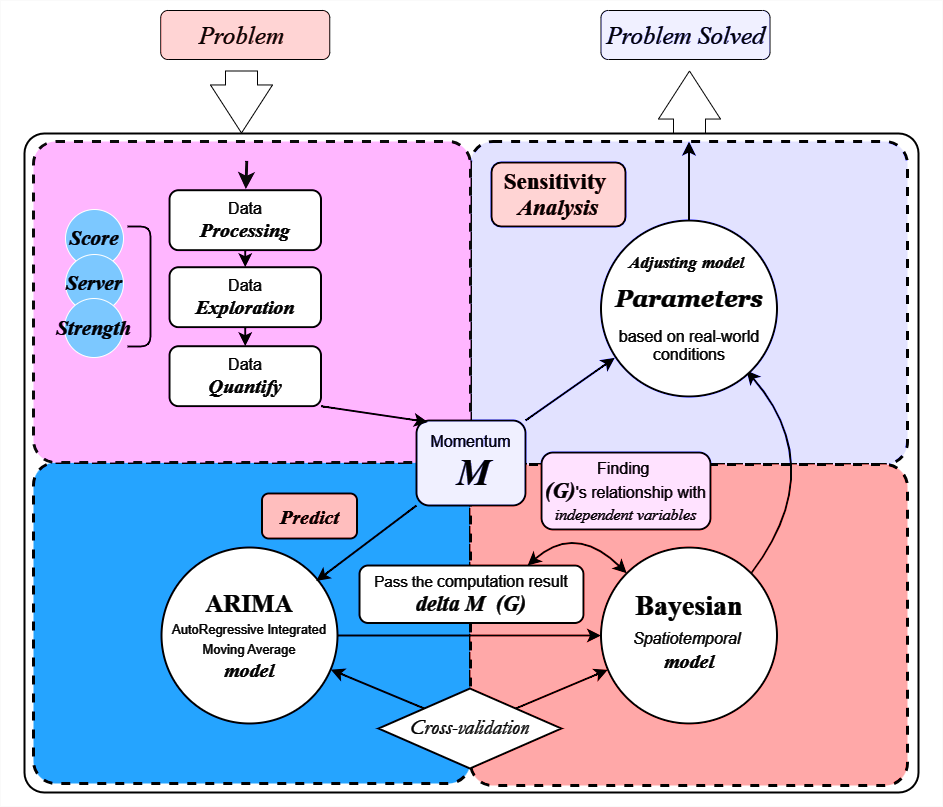
\includegraphics[width=.6\textwidth]{Figureflow.png}
\caption{Work Flow}\label{fig:ourwork}
\end{figure}


\section{Preparation of the Models}
\subsection{Assumptions}
Based on the simplifications made to the model, we have established the following reasonable assumptions:
\begin{enumerate}[\bfseries 1.]
	\item Momentum influences the progression of the match, thereby affecting the outcome, while other aspects of players' performance also impact the result. This assumption effectively connects player performance, match outcomes, and momentum, thereby better defining and quantifying momentum.

	\item The difference in skill level among participating players is relatively small, and match outcomes are not directly determined by a significant gap in absolute strength but are related to changes in momentum for both sides. This assumption ensures that momentum's influence on the match is not affected by external factors.

	\item Players' momentum fluctuates, allowing momentum to be correlated with pivotal moments in the match. This assumption enables the association of momentum with critical turning points in the game.

	\item Momentum is related to the psychological state of the players. When players are on a winning streak or serving, they have greater confidence in their next shot, leading to a noticeable increase in momentum. This assumption clearly identifies factors that have a significant impact on momentum, facilitating the quantification of momentum.
\end {enumerate}

By adopting these assumptions, the model simplifies the complex dynamics of the game while still capturing essential aspects related to momentum and player performance.

\subsection{Notations}
The primary notations used in this paper are listed in Table \ref{tb:notation}.

% 三线表示例
\begin{table}[!htbp]
\begin{center}
\caption{Notations}
\begin{tabular}{cl}
	\toprule
	\multicolumn{1}{m{3cm}}{\centering \textbf{Symbol}}
	&\multicolumn{1}{m{8cm}}{\centering \textbf {Definition}}\\
	\midrule
	$\Delta M$&the players' momentum difference at a given moment\\
	$\delta M$&the $\Delta M_t$ difference between adjacent time points\\
	$ G $ & $ \delta M $\\
	$ P $ & the probability of one player gaining an advantage \\
	\bottomrule
\end{tabular}\label{tb:notation}
\end{center}
\end{table}

\section{Model 1:Momentum Quantification and ARIMA Integration}

We integrated momentum, a comprehensive assessment derived from various aspects of a player's performance, with ARIMA forecasting model. Quantifying momentum allows us to reflect players' competitive status to facilitate rapid adjustments. By analyzing momentum changes and trends, we can make relatively accurate predictions about the progression of the match. Therefore, we first considered factors that significantly influence momentum and derived a criterion to evaluate momentum. Subsequently, we used the ARIMA model to forecast the match's progression and ultimately identify the turning points where one side transitions to the other.

\subsection{Construction of Momentum Evaluation Formula}

Firstly, we consider that players gain confidence during winning streaks, allowing them to utilize their full potential. However, this effect diminishes as their confidence reaches a certain level. Moreover, the outcome of the previous point directly influences a player's subsequent performance. Additionally, we observe that players have a higher winning rate when serving compared to when receiving. However, if a player makes an error on their first serve, they face the risk of losing the point directly on their second serve, leading to a more cautious approach. Furthermore, facing break points or multiple failed serves increases psychological pressure on players, negatively affecting their momentum. Also, we notice a strong correlation between players' fatigue levels and their performance; as fatigue increases, performance declines. The fluctuation in momentum at different moments reflects the fluctuation in player states, which often impacts the match's progression. Consequently, we find a strong correlation between the difference in momentum at different times and the match outcome.

To investigate the impact of changes in momentum for both sides on match fluctuations, we denote the difference in momentum between two players at the same moment as $\Delta M_t$, which reflects differences in player states. Then, we define the difference in $\Delta M_t$ at different time points as $\delta M$. Since the momentum of both players is not necessarily equal at a specific time point, $\delta M$ reflects changes in the difference in momentum between the two players. If $\delta M$ is positive, it indicates a higher likelihood of winning the match. After fitting operations, we observe a strong correlation between $\delta M$ and subsequent victories.

\begin{equation}\label{eq:k1}
K_1=1.3-0.3\cdot\exp\left(1-x\right)
\end{equation}

\begin{equation}\label{eq:k2}
K_2=victouy?1:-0.9
\end{equation}

\begin{equation}\label{eq:p1}
P_1=\left\{
\begin{aligned}
1.2 \to is \ server\\
0 \to not \ server 
\end{aligned}
\right.
\end{equation}

\begin{equation}\label{eq:p2}
P_2 = \left\{
\begin{aligned}
0.75 \to fist \ fault \\
1 \to fist \ succeed 
\end{aligned}
\right.
\end{equation}

\begin{equation}\label{eq:dq}
\delta Q =- \frac {\sum\limits_{i=1}^n (distan_1-distan_2)}{sum}
\end{equation}

\begin{equation}\label{eq:preM}
preM_{t+1}=preM_{t}+\frac{\prod\limits_{i=1}^n K_i+\prod\limits_{j=1}^m P_j}{2}
\end{equation}

\begin{equation}\label{eq:DELM}
\Delta M_t = preM_{1t} - preM _{2t}+\delta Q
\end{equation}

\begin{equation}\label{eq:dDELM}
 \delta M = \Delta M_{t+1}-\Delta M_{t}
\end{equation}

As for the weights of $\prod\limits_{i=1}^n K_i$ and $\prod\limits_{j=1}^m P_j$, we later utilized sensitivity analysis.

Going forward, we will use MDELM to represent $\Delta M$ and dDELM for $\delta M$ for brevity.

\subsection{Testing of the Momentum Evaluation Formula}

We plotted the curve of $\Delta M$ against time using the data from the match 2023-wimbledon-1701. It is easy to observe that if the subsequent point is a red dot, $\Delta M$ between the previous and subsequent points decreases; if the subsequent point is a blue dot, $\Delta M$ increases. That is, when $\delta M$ is positive, Player 1 has a high probability of winning the match. When the sign of $\delta M$ changes, the trend of winning the match shifts from one player to the other.

\begin{figure}[H]
\centering
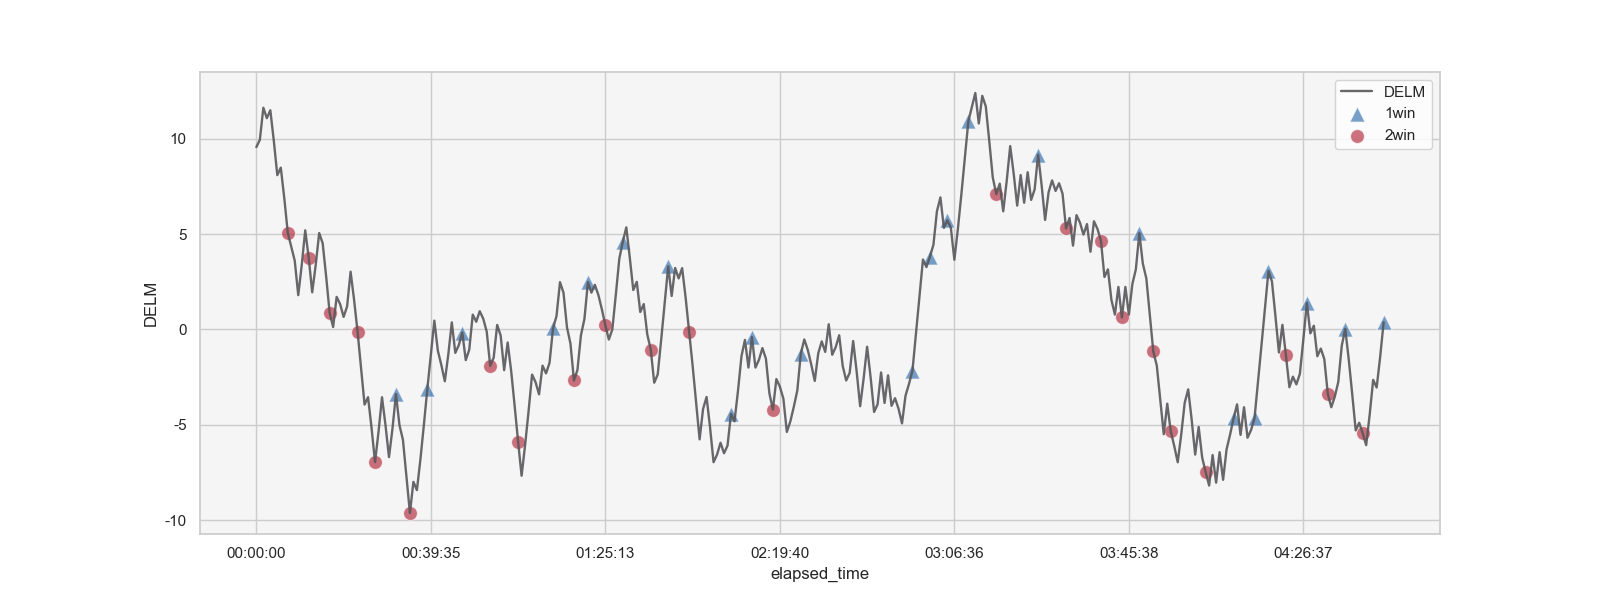
\includegraphics[width=\textwidth]{DELM1.png}
\caption{The result of $\Delta M$}\label{fig:DELM1}
\end{figure}

We conducted a Pearson correlation analysis between the DELM, dDELM data, and whether the player won, resulting in a heatmap.

\begin{figure}[H]
\centering
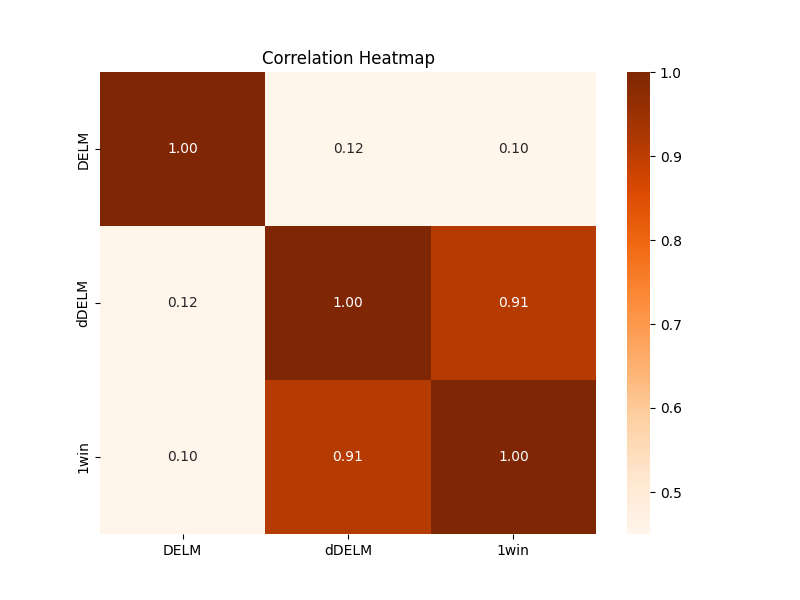
\includegraphics[width=.6\textwidth]{heatmap.png}
\caption{HeatMap}\label{fig:heatmap}
\end{figure}

We found a correlation coefficient of 0.91 between $\delta M$ and the outcome of the match. Therefore, we can conclude that the fitting of dDELM, representing $\delta M$, is effective.$^{[3]} $

\subsection{Predicting Player Performance with ARIMA and $\delta M$}

We utilize the momentum evaluation formula to calculate the value of $\delta M$. Given $\delta M$'s strong correlation with match results and player performance, we employ the ARIMA model to process $\delta M$ and predict the progression of the match.

\subsubsection{Explanation of the ARIMA Model}

The ARIMA model (Autoregressive Integrated Moving Average) is a widely used method for time series forecasting analysis. To enhance prediction accuracy, the ARIMA model combines autoregression (AR) and moving average (MA) methods and integrates differencing (I) to handle the characteristics of non-stationary time series. Because the ARIMA model can capture various autocorrelation structures in time series, it is particularly suitable for short-term forecasting.$ ^{[4]}$ Researchers can simulate and forecast corresponding time series data by adjusting the parameters (p, d, q), where p represents the order of autoregression, d represents the differencing level, and q represents the order of the moving average.

\subsubsection{Fitting with the ARIMA Model}

We first define the 'check' class, which receives the differencing flag and handles it. Additionally, it conducts unit root (ADF test) and white noise tests to evaluate the stationarity and randomness of the data. Then, we use the arma\_order\_select\_ic method to select the orders of the ARIMA model that best fit the data based on the AIC and BIC criteria. Finally, we fit the data with the ARIMA model, plot the autocorrelation and partial autocorrelation graphs, make predictions, and compare the predicted results with the actual values. We calculate the mean absolute error of the predictions and analyze the normality of the residuals to evaluate the model. We also define the 'generate' class, which first splits the dataset into training and testing sets. Then, it analyzes trends and changes by computing and comparing the differences between actual and predicted data.

Below are the results of the ADF test:

\begin{table}[H]
\begin{center}
\caption{ADF Test Results}
\begin{tabular}{cccccccc}
	\toprule
	\textbf{Variable} & \textbf{Differencing Order} & \textbf{t} & \textbf{P} & \textbf{AIC} & 			\multicolumn{3}{c}{\textbf{Critical Values}} \\
	\midrule
	 & & & & & \%1 &\%5 & \%10 \\
	\midrule
	 & 0 & -3.413 & 0.011** & 1040.585 & -3.451 & -2.871 & -2.572 \\
	DELM & 1 & -16.172 & 0.000*** & 1044.606 & -3.451& -2.871& -2.572 \\
	 & 2 & -9.439 & 0.000*** & 1073.071 & -3.452& -2.871& -2.572 \\
	\bottomrule
	\multicolumn{8}{c}{Note: ***, **, and * respectively represent significance levels of 1\%, 5\%, and 10\%.}
\end{tabular}\label{tb:adf}
\end{center}
\end{table}

The result of this sequence test shows that, based on the variable DELM: when the differencing order is 0, the significance level P-value is 0.011**, indicating significance at the 1\% level. We reject the null hypothesis, indicating that the sequence is a stationary time series. Therefore, we determine our d parameter to be 0.

Next, we use ACF and PACF plots to select the p, d, and q parameters for ARIMA.

\begin{figure}[H]
\centering
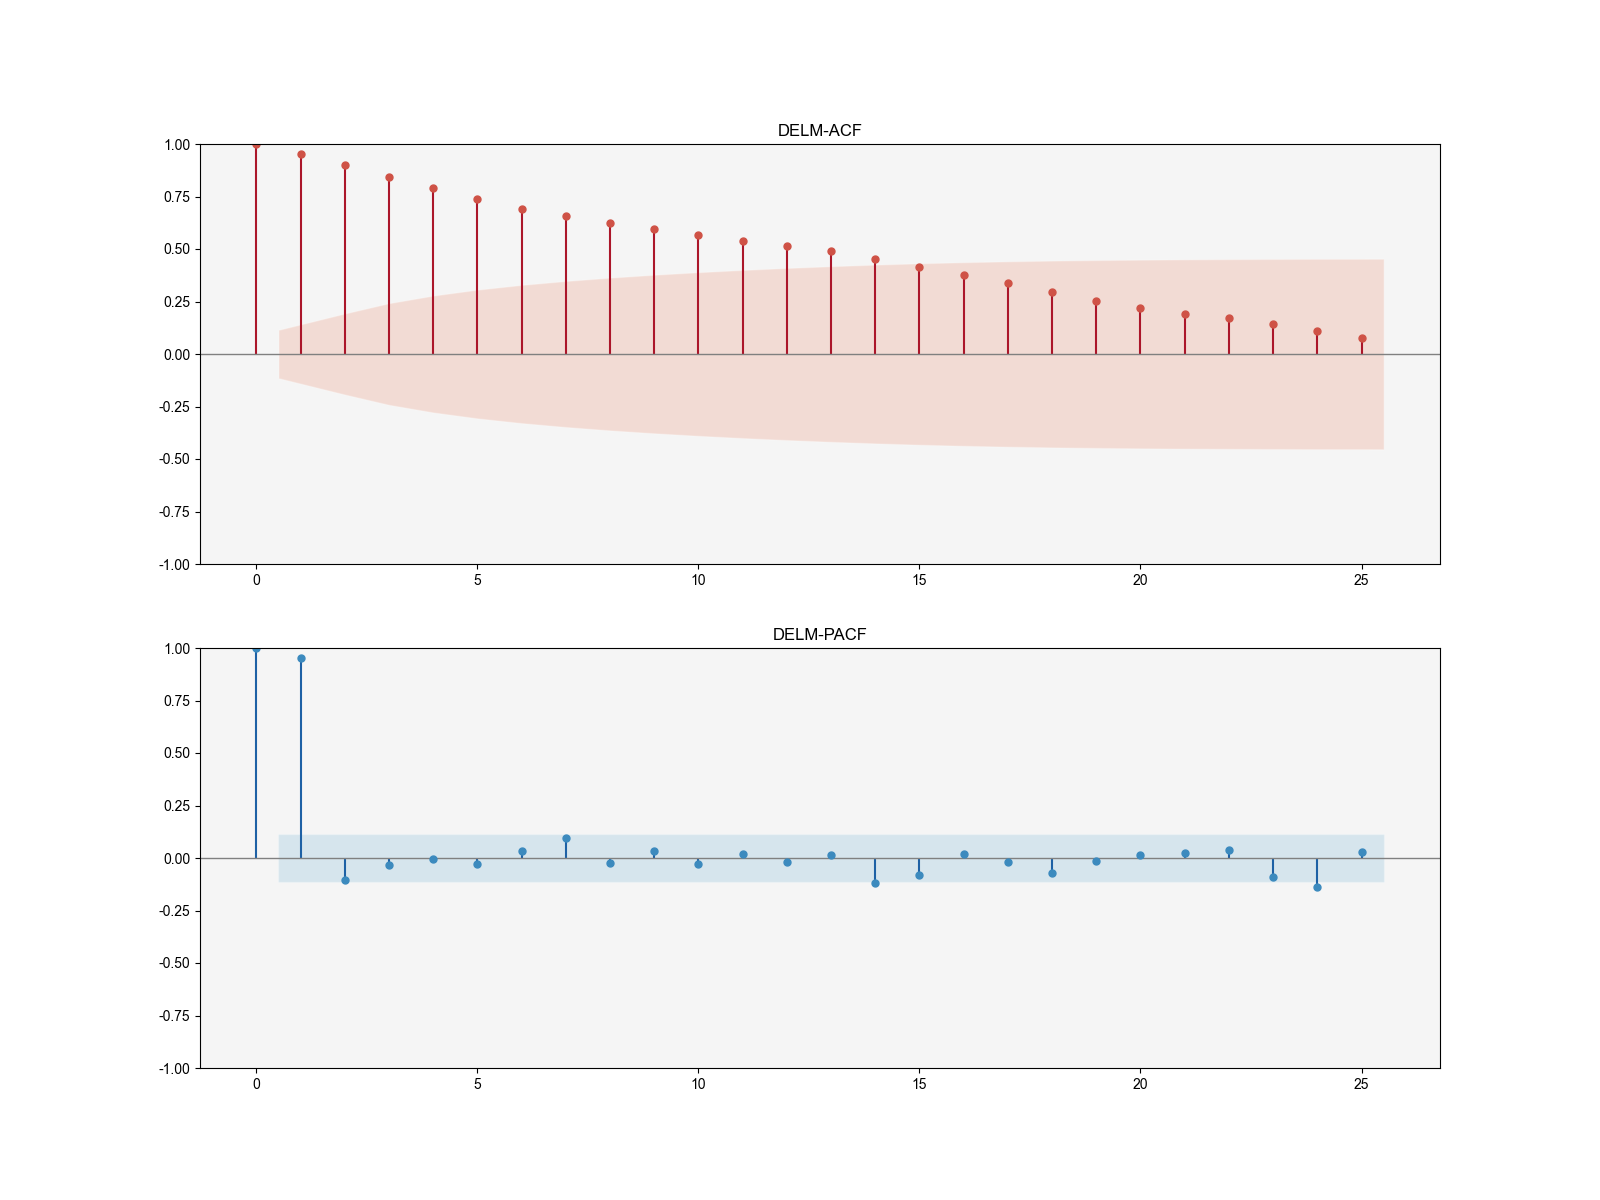
\includegraphics[width=.8\textwidth]{acfpacf.png}
\caption{ACF \& PACF}\label{fig:apacf}
\end{figure}

Referring to the images and using the AIC, BIC selection criteria, along with some adjustments, we have chosen the (1,0,4) parameters.

The formula for the model obtained using ARIMA(1,0,4) is as follows:

\begin{equation}\label{eq:arima}
\begin{split}
y(t)=0.027+0.938 \cdot y(t-1)+0.138 \cdot \varepsilon (t-1)+0.036 \cdot \varepsilon(t-2) \\
+0.033 \cdot \varepsilon(t-3)+0.035 \cdot \varepsilon(t-4)
\end{split}
\end{equation}

Subsequently, we obtained the fitting effect of the predicted values and actual values, and found that they closely matched the original data.

\begin{figure}[H]
\centering
\includegraphics[width=\textwidth]{arima\_show.png}
\caption{ARIMA}\label{fig:arima}
\end{figure}


\subsubsection{The forecast results using the ARIMA model}
The visualization of the forecast results is shown in the following figure, with the 95\% confidence interval shaded in gray. We have achieved short-term forecasting, which can be used to determine the trend of winning or losing using $\delta M$.

\begin{figure}[H]
\centering
\includegraphics[width=\textwidth]{arima\_test.png}
\caption{ARIMA test}\label{fig:ariamtest}
\end{figure}

Seeing the satisfactory results, we proceeded to forecast the next 10 sets.

\begin{figure}[H]
\centering
\includegraphics[width=\textwidth]{arima\_predict.png}
\caption{ARIMA predict}\label{fig:ariampredict}
\end{figure}

There is a downward trend, and we anticipate that the momentum of player 1 will be poor in the next match, leading to a loss. We will use dDELM to assess the degree of decrease in their momentum.

\subsection{The impact of momentum on the match results}

To demonstrate that the "momentum" we fitted has an impact on the results, we use ACF, PACF plots as references, along with a logistic regression model to analyze whether the previous $\delta M$ has an effect on the outcome.

\subsubsection{Logistic Regression$^{[5]} $ Model Explanation}

Logistic Regression is a statistical method widely used for predicting the probability of binary response variables. Its essence lies in mapping the output of a linear regression model to probabilities between 0 and 1 using a logistic or log-odds model.

The model is typically represented as:

\begin{equation}\label{eq:logistic}
\log\left(\frac{p}{1-p}\right) = \beta\_0 + \beta\_1X\_1 + \beta\_2X\_2 + \cdots + \beta\_nX\_n
\end{equation}

In the equation, $p$  represents the probability of the dependent variable (such as the probability of winning) taking the value 1. $ X_1$, $X_2$, $\ldots$, $X_n $ are the independent variables (explanatory variables), and $ \beta_0$, $\beta_1$, $\ldots$, $\beta_n $ are the model parameters.

\subsubsection{Using the Logistic Regression model to analyze the impact of $\delta M$ }

We referred to the ACF and PACF plots and observed autocorrelation showing a "tail" pattern. Since future values in a time series may be influenced by past values, the tail pattern implies strong correlation. Thus, we can preliminarily conclude that $\delta M$ has an impact on the outcome.

We first instantiated the `judge` class and then selected DELM and dDELM from the dataframe as independent variables (explanatory variables) and 1ifwin as the dependent variable (response variable). By adding a constant term to the independent variables, we fitted the logistic regression model.

Referencing the results of the Logistic Regression model:

\begin{table}[H]
	\centering
	\caption{Logit Regression Results}
	\begin{tabular}{lcccc}
		\toprule
		\textbf{Variable} & \textbf{Coefficient} & \textbf{Standard Error} & \textbf{z} & \textbf{P>|z|} \\
		\midrule
		\textbf{const} & -0.0142 & 0.113 & -0.126 & 0.900 \\
		\textbf{DELM} & -0.0679 & 0.025 & -2.742 & 0.006 \\
		\textbf{dDELM} & -0.0018 & 0.084 & -0.022 & 0.983 \\
		\bottomrule
	\end{tabular}\label{tb:logit}
\end{table}

In this model, the p-value for the variable DELM is 0.006, which is less than the commonly used significance level of 0.05. This indicates that the coefficient of the DELM variable is significantly different from zero. Therefore, it can be concluded that the DELM variable has a significant impact on the dependent variable.

\begin{figure}[H]
	\centering
	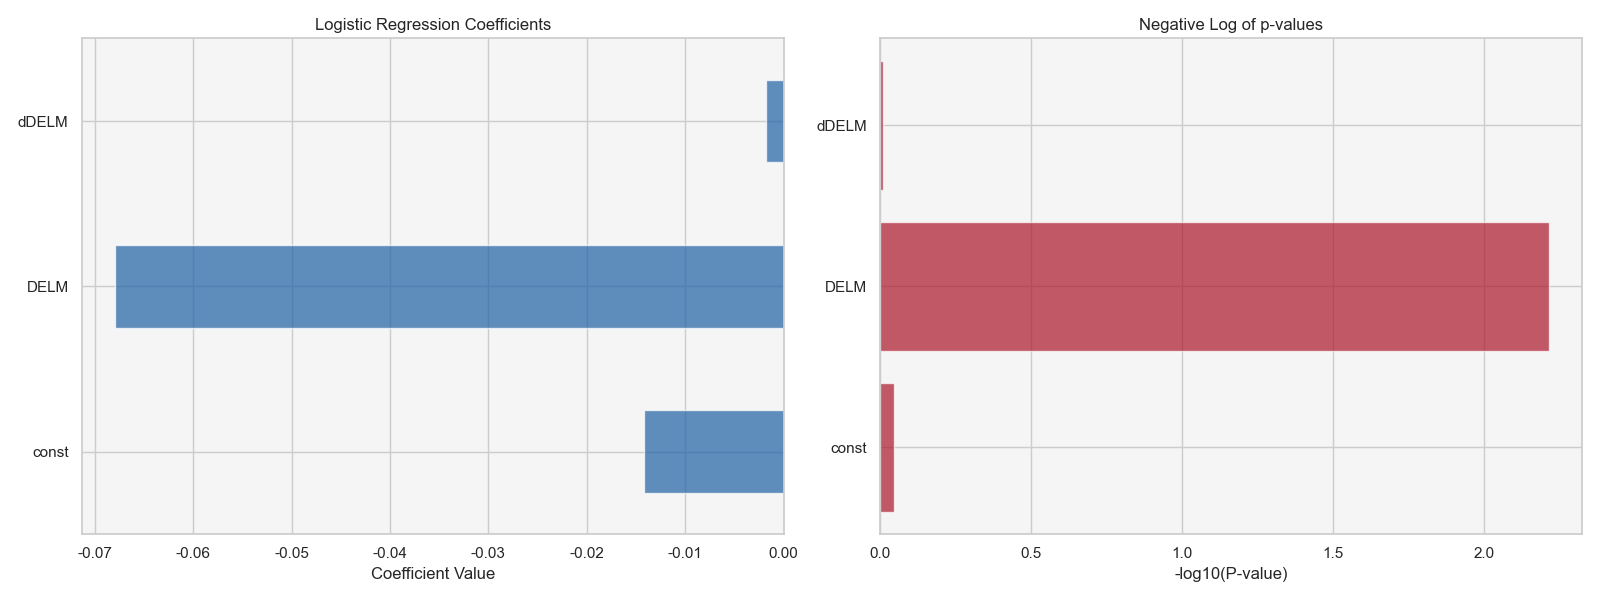
\includegraphics[width=\textwidth]{p-value.png}
	\caption{p-value}\label{fig:pvalue}
\end{figure}

Therefore, we can conclude that the fitted DELM has a significant impact on the outcome of the match. This can refute the coach's idea.

\section{Model 2:Analysis and Evaluation Model Based on Bayesian Spatiotemporal Model}

\subsection{Characterization of the fluctuation probability in tennis matches}

Characterizing Factors Influencing Fluctuations in Tennis Matches

For both players and coaches, understanding the factors influencing fluctuations can better capture signs of momentum reversal. By changing strategies, namely the factors affecting fluctuations, one can shift the momentum of the tennis match in their favor.

Based on the conclusions of the momentum model described in the previous section, as shown in Figure 3.2-1, our momentum model exhibits strong fluctuations over time. Meanwhile, dDELM, the rate of change in momentum difference between both sides, implies the final outcome of the match. As depicted in Figure 3.2-2, the high correlation between dDELM and match results suggests that using dDELM as a criterion for assessing fluctuations in tennis matches is highly appropriate. Therefore, our aim to identify factors influencing fluctuations essentially involves determining the determinants of dDELM. For convenience, we refer to dDELM as the reversal factor, denoted as G.

Based on the dataset, we derive the distribution of all G, denoted as $\Omega$. We observe that G is roughly concentrated between four values, with a limited distribution range that is approximately symmetrical about the origin. Combining this with empirical assumptions, we hypothesize that the possible values of G for each player during the match are concentrated in the [-2, 2] interval, and roughly follow a "U"-shaped distribution about 0.


\begin{figure}[H]
	\centering
	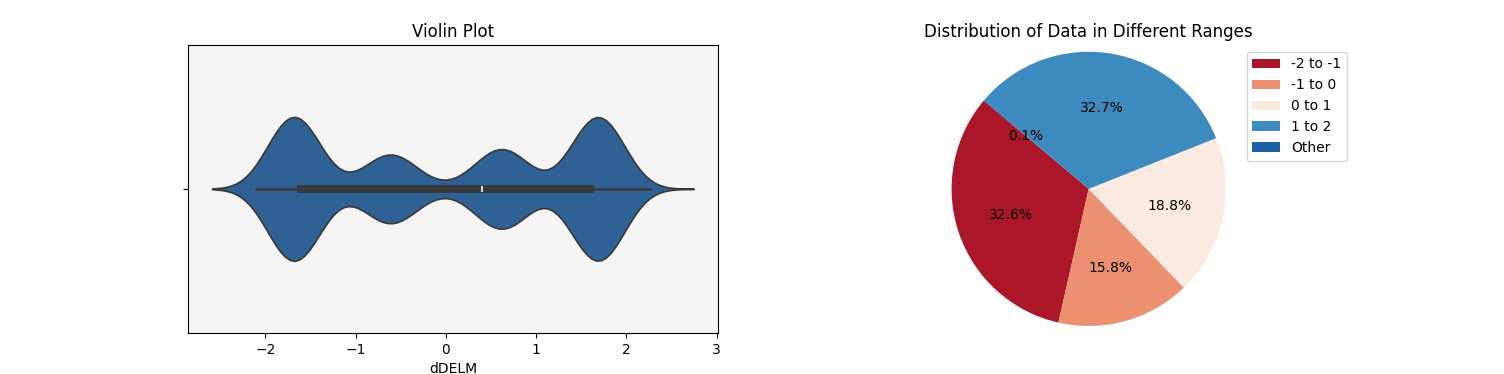
\includegraphics[width=\textwidth]{viovin.png}
	\caption{Violin plot \& Pie chart}\label{fig:vica}
\end{figure}

The fluctuations in tennis matches exhibit both temporal and spatial correlations, with players acting as spatial factors and match time serving as the temporal dimension, jointly determining the ups and downs of tennis matches. The Bayesian spatio-temporal model is a mathematical model established within the framework of Bayesian statistics to analyze the temporal and spatial information inherent in spatio-temporal data. It utilizes prior knowledge and conditional probabilities to compute the posterior distribution of parameters, with the most common method being Markov Chain Monte Carlo (MCMC) for computation. Considering the Bayesian spatio-temporal model's suitability for fitting time, space, and probability distributions (i.e., the probability of an event occurring),$^{[6]}\ ^{[7]} $  we use the log-logistic regression under the Bayesian spatio-temporal model to fit and analyze other variables.

\subsection{Correlating factors affecting match fluctuations}

\begin{figure}[H]
	\centering
	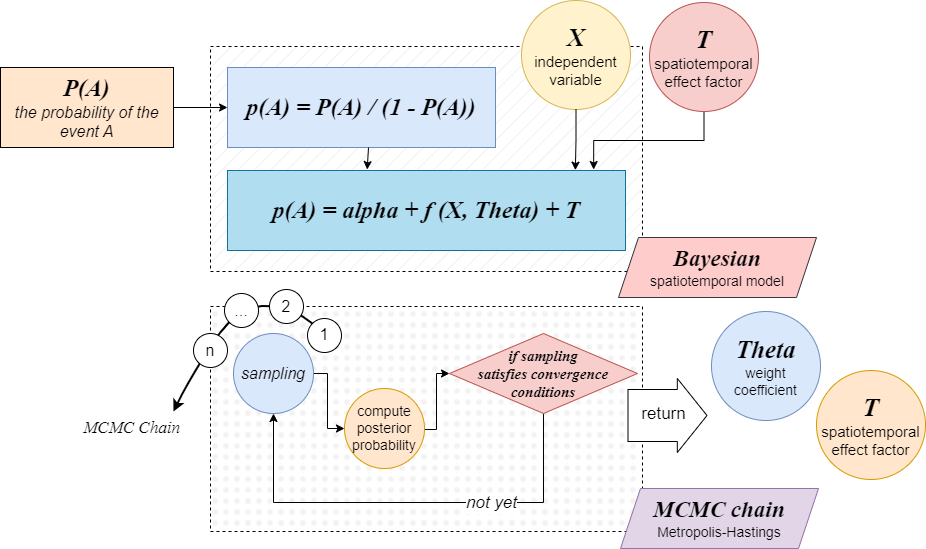
\includegraphics[width=\textwidth]{FigureModel.png}
	\caption{Model Logic Flowchart}\label{fig:figmo}
\end{figure}

Considering a model with random time effects in a single match, we can transform players' fluctuations during the game into the probability of one player gaining an advantage by the following means.

\begin{equation}\label{eq:g}
	G_t < 0
\end{equation}

Obviously, when player 1 is at a disadvantage, and vice versa when

\begin{equation}\label{eq:gt}
G_{t}\cdot G_{t+1} < 0
\end{equation}

we consider that a reversal of fortune has occurred. Let $\Omega$ represent the sample space composed of all G, and we use the relative distribution of G to represent the probability of player 1 having an advantage.

\begin{equation}\label{eq:gt}
P(t) = \frac{n(i|G_i\in[G_{min},G_t])}{n(\Omega)}
\end{equation}

We found that in the bipolar distribution of G, when a player is at the lower (upper) bound, the probability of a comeback (being counterattacked) is also lower. This aligns with our everyday understanding and the sample space formed by the G depicted in the above figure.

To explore the relationship between G and other variables we are interested in, we can, based on log-logistic and Bayesian spatiotemporal model theories, calculate the probability distribution column P for all G. Subsequently, we can use this P value in regression analysis with the other variables we want to explore and introduce.

Based on the log-logistic and Bayesian spatiotemporal models, we obtain the equation:

\begin{equation}\label{eq:gt}
	logit P(i) = \alpha + f(X(i),\Lambda) + \tau_i
\end{equation}

to fit probability values
In this equation:

i —  data point
$\tau_{i}$ — Time random effect factor
X — Matrix of independent variables 
f — Quadratic polynomial
$\Lambda$ — Weighting matrix

For variables representing two players, such as P1\_Distance\_Run and P2\_Distance\_Run, we can eliminate the influence of spatial random variables on the coefficients by taking the difference.

For categorical variables, such as the 5 different serving methods in Serve\_Width, which are not numerical, to account for the impact of different serving methods on P, we will use the method of dummy variables. For each sample point, we use a matrix [x\_0, x\_1, x\_2, x\_3, x\_4], where x\_i $\in$ {0,1} represents Serve\_Width, and x\_i indicates whether the i-th serving method is used. To assess the effects of different serving methods, i.e., when measuring the effects under different values of x\_i, we construct a coefficient matrix $\Theta$ = [k0, k1, k2, k3, k4] to evaluate the individual effects of x\_i. The advantage of this approach is that it can reduce errors in the analysis of the causes and effects of independent variables due to data processing issues.

Furthermore, variables like Serve\_Width can exhibit fluctuations in their impact on P depending on the Server. Therefore, we first appropriately handle the values of Server, mapping them to {-1,1}. Subsequently, we construct interaction terms between Server and variables affected by its fluctuations, such as Serve\_Width, to reduce this influence.

To estimate the coefficients in the logistic regression expression, i.e., the coefficient matrix in the expression, we use an MCMC chain for regression analysis. After properly processing the dataset, it is imported into WinBUGS14 for iteration. When the number of iterations is set to 10,000, the obtained coefficients are as follows:

The weight coefficients obtained from WinBUGS14 roughly follow a normal distribution, aligning with the model's assumptions. The MCMC chain converges, indicating a good fit.

Some of the parameter confidence intervals include zero, indicating that the effect of those independent variables on the model is not significantly pronounced, such as the intercept; or it could be that the variable itself exhibits variability, as in the case of Return\_Depth.

On the other hand, variables with confidence intervals (CI) excluding zero, especially those with narrow upper and lower bounds, exhibit a stronger and more pronounced impact on the model, such as the serving side. According to our model, the serving side plays a significant role in numerous interaction terms, influencing variables like the serving technique to a considerable extent.

\begin{figure}[H]
	\centering
	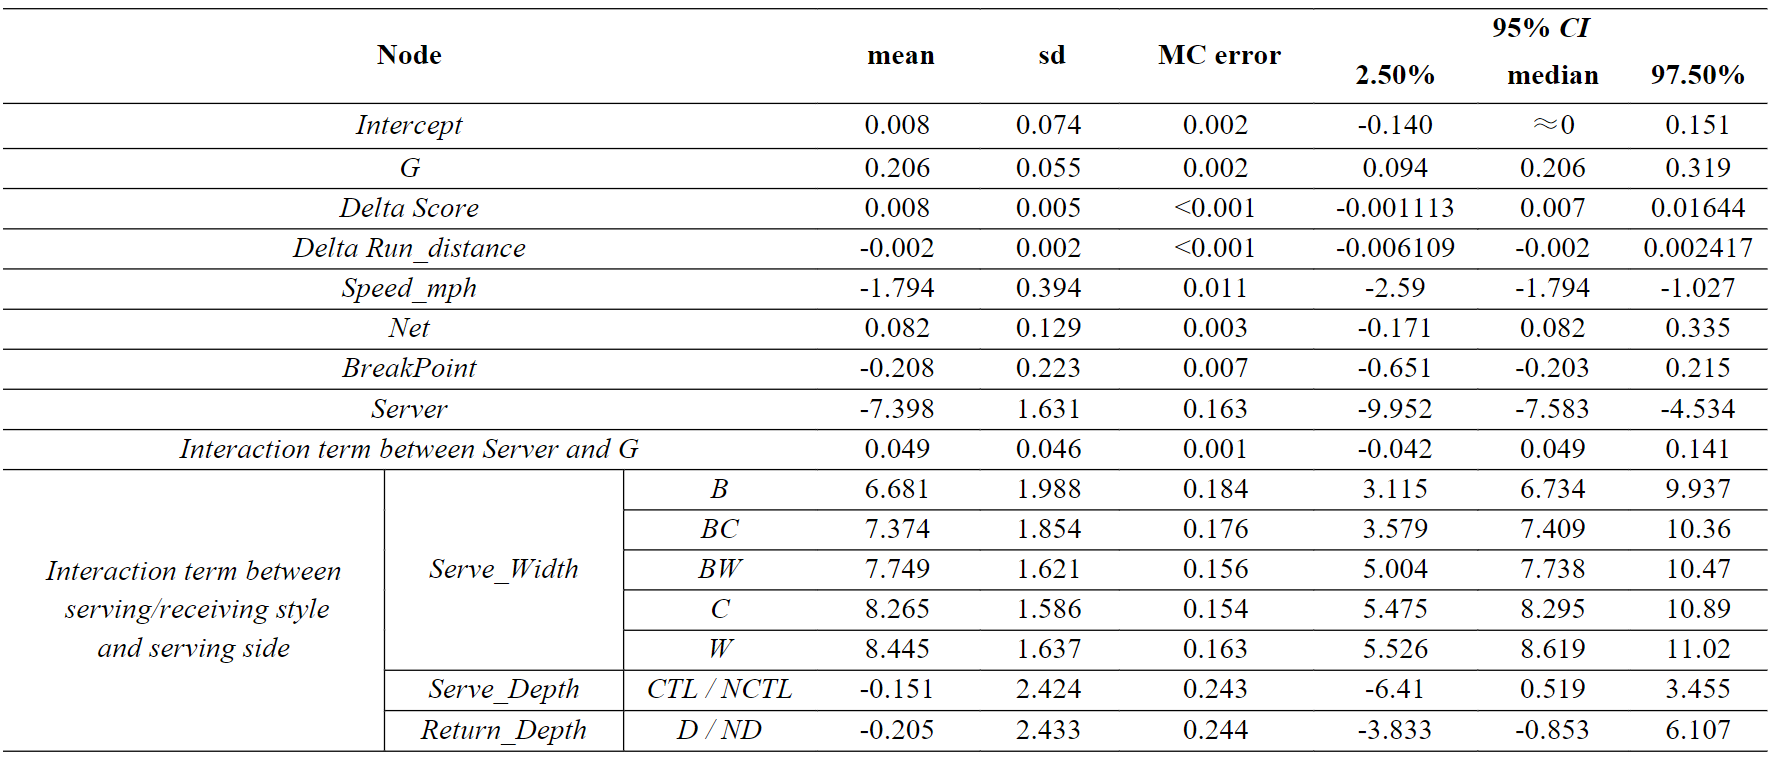
\includegraphics[width=\textwidth]{char1.png}
	\caption{Correlation Coefficient}\label{tb:char1}
\end{figure}

\subsection{Discussion on Model Fit Accuracy}

We analyzed the distribution of the time random effects factor, represented by the mean (red line), and its 95\% confidence interval (yellow line), as depicted in the graph below. From the plot, we observe a significant fluctuation in the time factor over time, suggesting the rationality of the time random effects factor we have set.

\begin{figure}[H]
	\centering
	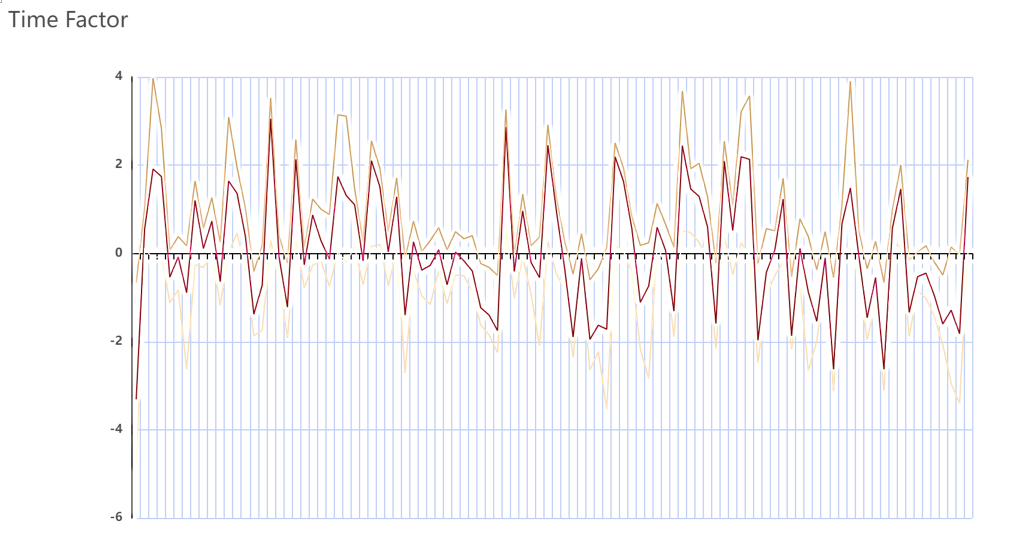
\includegraphics[width=\textwidth]{timefactor.png}
	\caption{Time Factor}\label{fig:timefactor}
\end{figure}

After obtaining the coefficient matrix, intercept, and time random effects factor, we proceeded to predict P, resulting in the predicted values (pre). The fitted graph is shown below, with Point\_no on the horizontal axis and probability values on the vertical axis.

\begin{figure}[H]
	\centering
	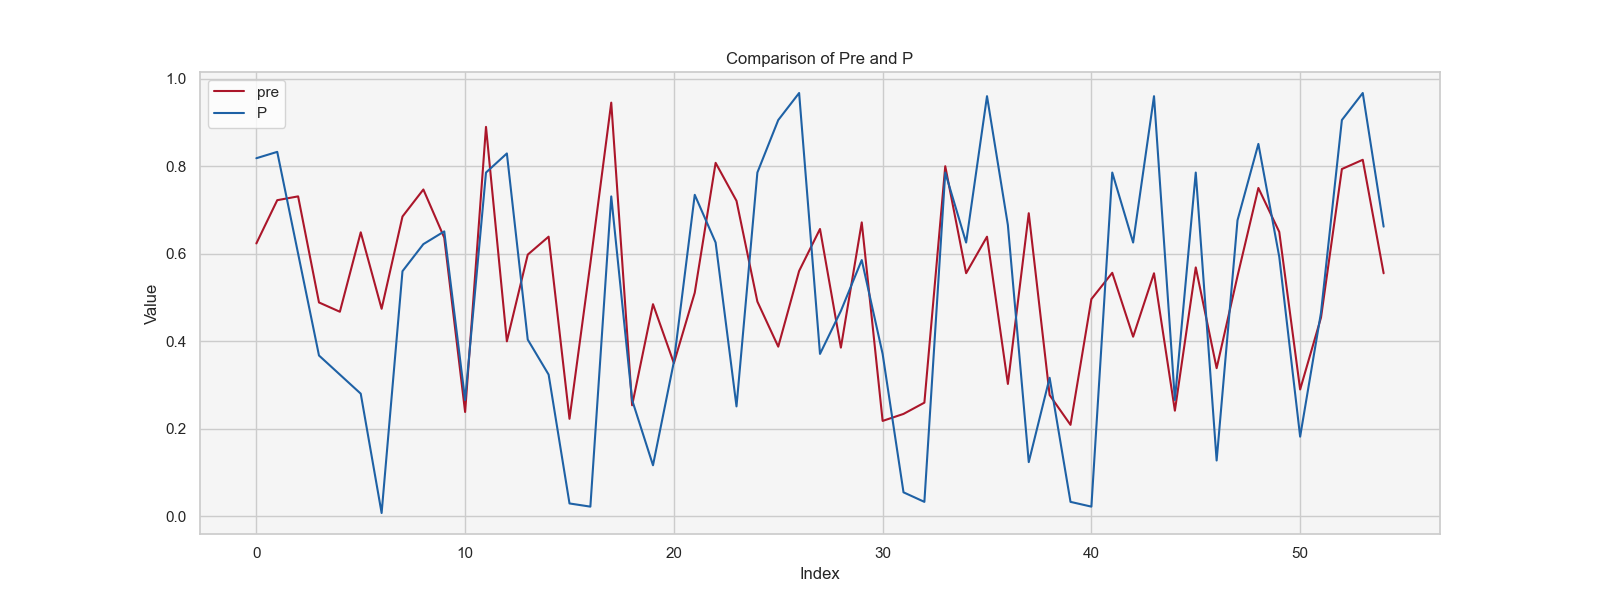
\includegraphics[width=\textwidth]{qwer.png}
	\caption{Level of Fit}\label{fig:qwer}
\end{figure}

\subsection{Recommendations Based on the Impact of Various Factors on Matches}

Given the numerous uncontrollable factors on the court, such as the opponent's serve direction and intensity, to provide players with actionable recommendations for altering the situation, we should focus on measures they can effectively execute in response to the next ball. For instance, adjustments in serving posture or receiving stance. Utilizing the model, we calculate the change in the probability variable ($\Delta P$) for each specific scenario. By determining the distribution proportion where $ \Delta P $ > 0, we obtain a probability distribution table indicating their likelihood of changing the game situation based on altering different factors.

When player1 is the server (with 'Return\_Depth' column indicating the opponent as the returner), the calculation yields:

\begin{figure}[H]
	\centering
	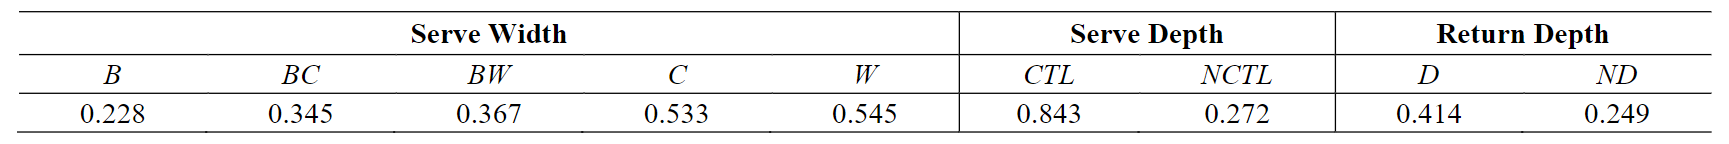
\includegraphics[width=\textwidth]{char2.png}
	\caption{Suggestions}\label{tb:char2}
\end{figure}

This table illustrates that when the player is serving, choosing strategies C, W, and CTL can increase the probability of scoring. On the other hand, when receiving, opting for return strategy D can enhance the likelihood of scoring.

%Based on the comprehensive model discussed above, when a tennis player faces a new opponent, I propose the following recommendations to help the player quickly adjust their state and perform at their best. Firstly, it is essential to analyze one's historical energy fluctuations during matches. Reviewing situations where quick momentum gains were achieved and identifying factors leading to a decrease or loss of energy can provide valuable insights. Learning from these experiences allows for the optimization of personal skills and tactics.

%Simultaneously, pre-match physical and psychological preparation remains crucial. Understanding the opponent's playing style beforehand and formulating specific game strategies based on their tactical habits is vital. Concurrently, intensifying training in certain technical aspects, such as improving serve quality and baseline endurance, ensures the ability to maintain high-intensity performance on the court.

%Lastly, possessing strong mental resilience is crucial. Believing in oneself to handle various challenges when trailing in score or facing unexpected errors is essential. Maintaining composure, controlling emotions, and minimizing the impact of consecutive losses on personal energy are vital aspects to swiftly regain momentum and enter a peak state during matches.

\section{Model 3: Momentum Evaluation Based on Cross-Validation Model}

\subsection{Testing the Universality of the Model}

With a relatively good fit obtained in the third question, to assess how well the model can predict fluctuations in matches, we employ cross-validation techniques. Leave-One-Out (LOO) cross-validation is a straightforward yet effective method. In LOO cross-validation, one sample is retained as the test set each time, while the remaining samples serve as the training set. This means that for a dataset containing n samples, the model is trained and evaluated n times, using n-1 samples for training in each iteration and testing with the remaining one sample.

The primary advantage of LOO cross-validation is its ability to make the most use of the data for model evaluation, as each sample is used for testing. However, its drawback lies in the relatively high computational cost, especially for large datasets, as it requires training a substantial number of models.

First, we compute differences for data processing and preparation. Then, we use r2\_score as the evaluation metric. Finally, by sequentially using each file as the test set and the rest as the training set, we assess the model's generalization ability on different datasets.

The accuracy of the prediction model is illustrated in the following figure, with an average accuracy value of 93.17\%. This indicates that our model performs relatively well in predicting fluctuations in matches.

\begin{figure}[H]
	\centering
	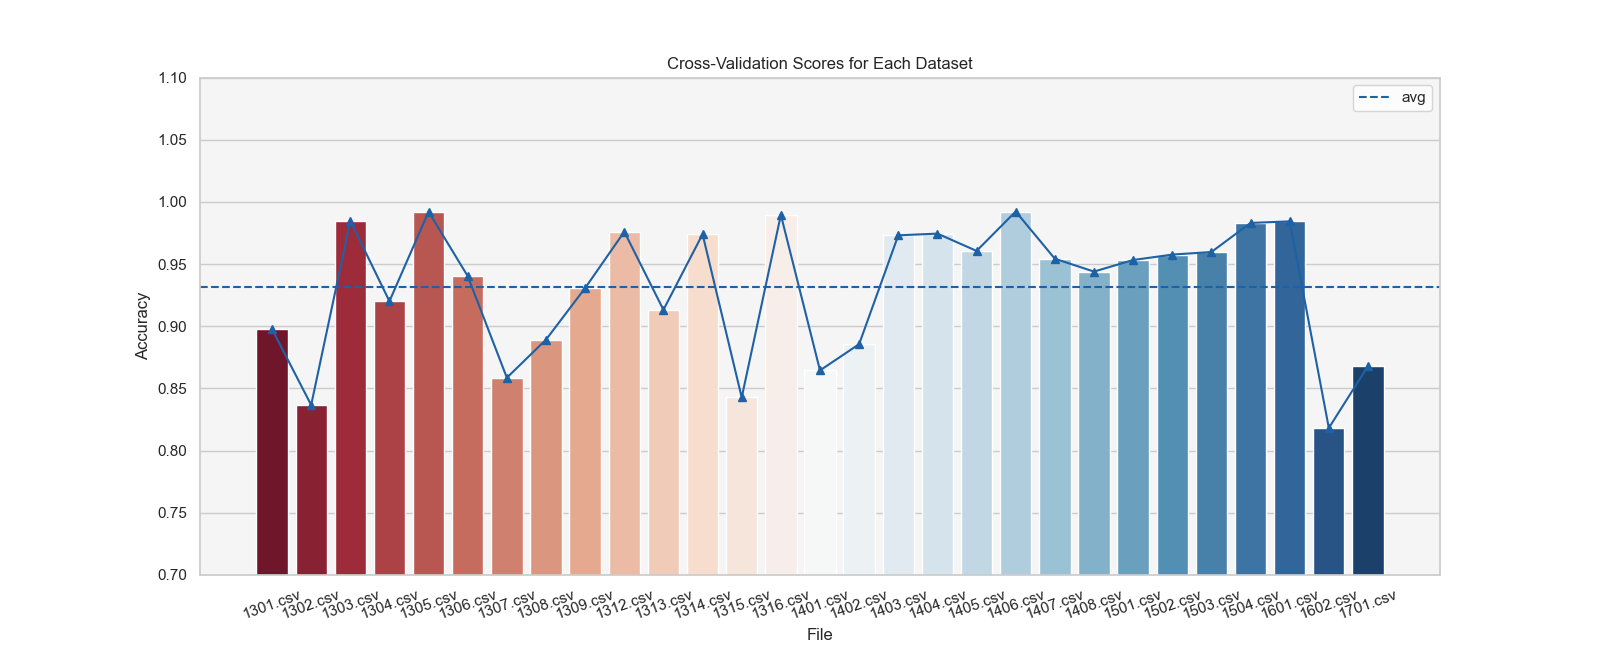
\includegraphics[width=\textwidth]{crosstest.png}
	\caption{Accuracy}\label{fig:crosstest}
\end{figure}

\subsection{Enhancing the Model by Incorporating Relevant Factors}

Based on our model and the observed fitting results, there are areas for improvement. The model exhibits a lag in predicting certain data and appears insensitive to data with low volatility. For a more comprehensive model in future development, we can consider incorporating spatiotemporal random effects for various match time points, especially when dealing with multiple events. I suggest including the following factors into consideration.

\begin{enumerate}[\bfseries 1.]
	\item The world rankings and historical head-to-head records of the two players: From the first model, we observe a significant correlation between changes in momentum and consecutive victories, as well as the outcome of the previous match. Both factors play a crucial role in boosting a player's confidence and maintaining a good competitive state.
	\item Surface conditions: Different playing surfaces affect the ball's bounce speed and height, as well as the players' movement on the court. Players adapt differently to surfaces like hardcourt, grass, and clay, which can influence the speed of their adaptation to the playing conditions.
	\item Audience and home court advantage: When players compete on their home turf, there is often more cheering and encouragement. These positive stimuli can quickly excite players and help them get into the groove more rapidly.
	\item Climate conditions: Temperature can alter the elasticity of the ball, humidity affects the ball's flight speed and bounce height, and both factors can contribute to increased fatigue for the athletes. These elements collectively influence a player's performance.
	\item Psychological expectations and pressure: While victory is a common goal for every player, each match holds different significance for individual participants. When a particular match is imbued with the potential to impact a player's career, the expectations and tension surrounding that match can be extraordinary. This pressure has the potential to either motivate the player to perform exceptionally well or adversely affect their psychological state, hindering them from getting into the desired mindset.
	\item Player's recent form: If a player is in a slump in their recent performances, both their confidence and momentum can be significantly impacted. Adjusting and bouncing back from such a phase is not an easy task in a short period.
	\item Tournament format: The rhythm control and energy allocation for players differ between formats like best-of-five sets and best-of-three sets. This variation can also influence their performance.
\end {enumerate}	

\section{Promotion of the Model}

\subsection{Rational Analysis of Momentum Indicator M in Women's Matches}

According to the literature, we analyzed the scoring performance of world-renowned female tennis players in the context of Breakpoints during the period from 2018 to 2019 under two conditions: 'whether serving' and 'whether leading in game points.' We observed that both being the server and leading in game points can enhance the scoring rate in crucial Breakpoint situations.$^{[8]}\ ^{[9]} $ The identity of the server remains a significant factor, showing a strong correlation with the momentum indicator M we constructed. Additionally, leading in game points can serve as another factor to assess the magnitude of momentum and be incorporated into our model.

\begin{figure}[H]
	\centering
	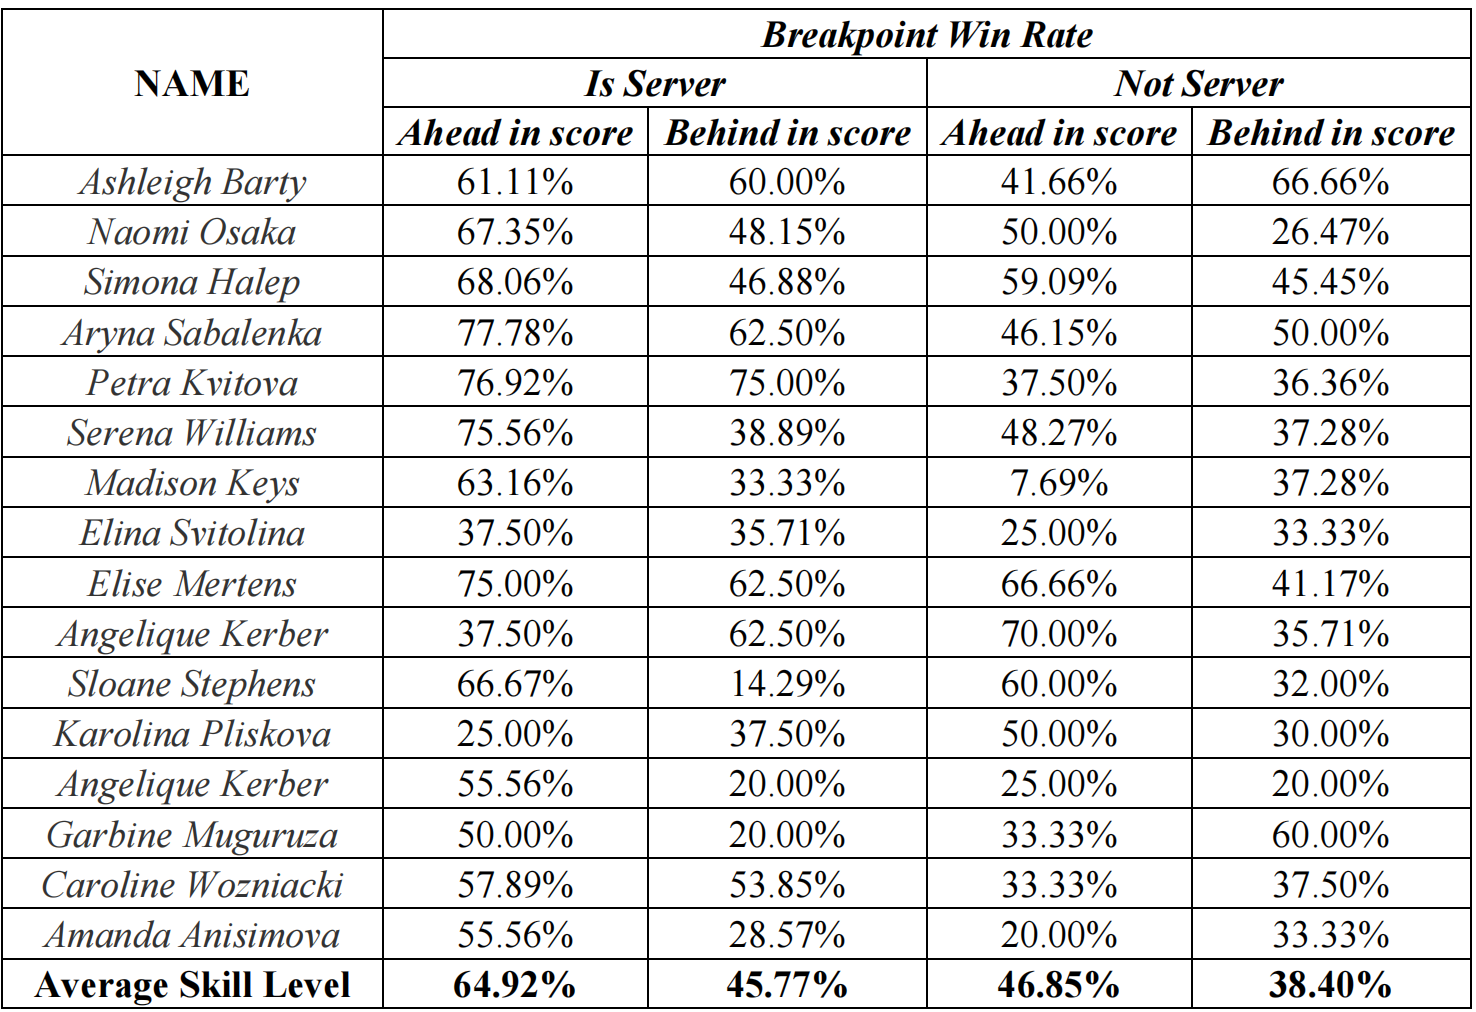
\includegraphics[width=\textwidth]{char4.png}
	\caption{Women Breakpoint Win Rate in Different Situations}\label{tb:char4}
\end{figure}

In fact, women's tennis matches share many factors influencing the course of the game with men's matches, such as the psychological state of players, technical abilities, and external environmental factors, all of which can impact the players' performance. However, the two cannot be entirely equated, and women's matches differ from men's matches in the following aspects:

\begin{enumerate}[\bfseries 1.]
	\item Differences in match duration and format
	\item Variances in physical factors leading to variations in ball speed and running distances
	\item Distinct preferences for winning through serving or receiving
	\item Disparities in the rate of physical recovery during consecutive matches
	\item Differences in handling psychological pressure
\end {enumerate}	

Due to the differing factors influencing momentum between men's and women's matches, simply transferring parameters obtained from men's matches into women's matches could potentially result in decreased predictive accuracy. However, employing a Bayesian spatio-temporal model with logit regression analysis can still recalibrate weight coefficients based on data from women's matches. Additionally, normalizing the data can mitigate biases arising from differences in average match duration and running distances between the two types of matches.

\subsection{Analysis of the Rationality of Momentum Indicator M in Different Court Conditions}

\begin{figure}[H]
	\centering
	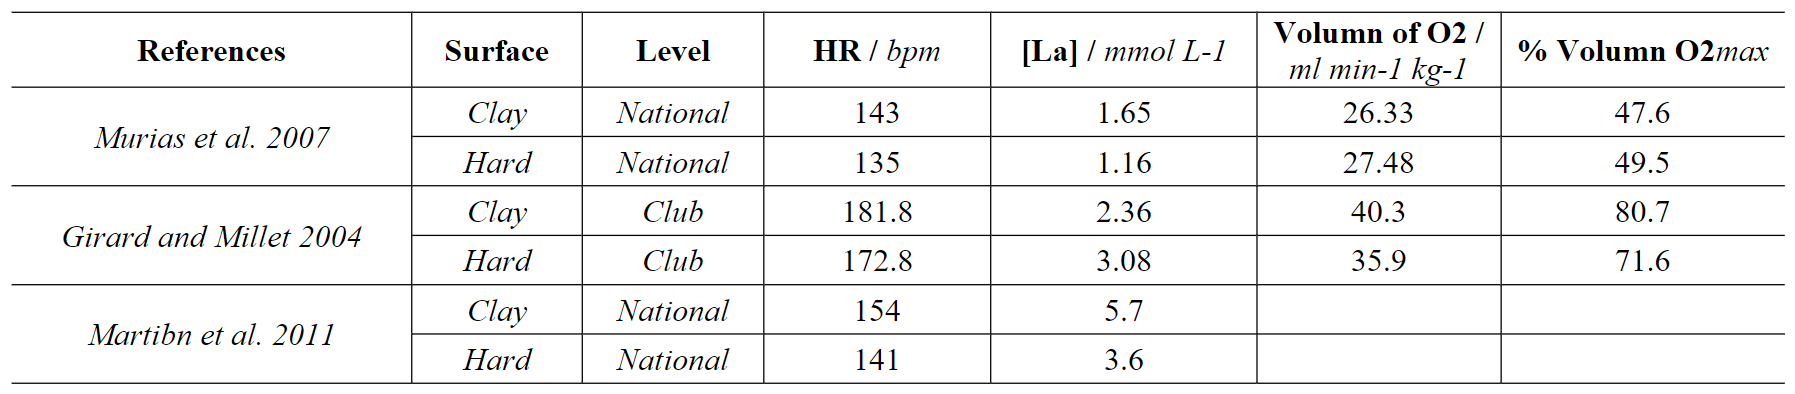
\includegraphics[width=\textwidth]{char3.png}
	\caption{Geographical Variations}\label{tb:char3}
\end{figure}

According to the literature, different playing surfaces represent distinct spatial environments. For instance, the oxygen content in the environment of club competitions is relatively high, which may have an impact on the players' stamina. The differences between gravel and hard surfaces also manifest in varying levels of physical activity, reflected in heart rate (HR). Therefore, we conclude that different spatial environments can influence serving, receiving, running distances, and even the athletes' physical fitness.$^{[10]} $

To mitigate these influences, we can incorporate spatio-temporal effect factors into the model expression. This involves adding factors to characterize random effects in different playing environments. By obtaining fitted values for these factors, the model's generalization capability is expected to be enhanced.

\subsection{Rational Analysis of Momentum Indicator M in Table Tennis Matches}

According to the literature, there is a strong correlation between the momentum value in table tennis matches and the serving side, serving methods during the serving and receiving phases, as well as the hitting methods during the receiving phase.

\begin{figure}[H]
	\centering
	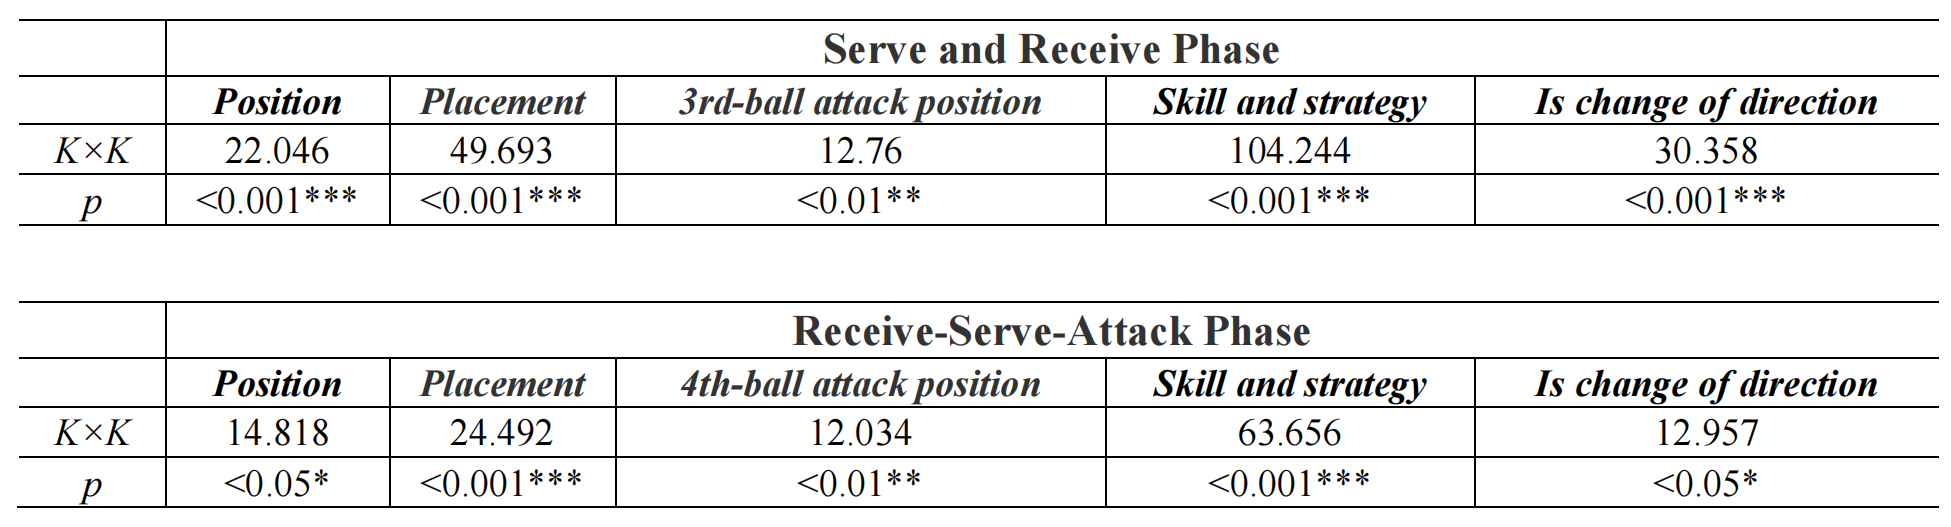
\includegraphics[width=\textwidth]{char5.png}
	\caption{Independence Test for Chi-square Plots}\label{tb:char5}
\end{figure}

Thus, we observe that, similar to tennis matches, the serving side, serving methods, hitting techniques, time sequence, and other factors continue to influence the momentum indicator M. Therefore, it remains reasonable to use factors such as (Score, Server) to characterize M. From the aforementioned data, it is evident that the winning strategies in table tennis have a stronger correlation with tactics compared to tennis. Hence, there is a greater need to amplify and refine the factor of 'strategy' and incorporate it into the logistic regression expression for M.

\section{Sensitivity Analysis}

We adjust the weights of $\prod\limits_{i=1}^n K_i$ and $\prod\limits_{j=1}^m P_j$. Let's assume the weight of $\prod\limits_{i=1}^n K_i$ is denoted by $\alpha$, and the weight of $\prod\limits_{j=1}^m P_j$ is $2 - \alpha$.

Then, through sensitivity analysis:

In the generation of accuracy, two methods, Kendall and Pearson, were employed to assess data correlation. These two methods are commonly used in statistical analysis to measure the correlation between two variables, especially for evaluating the rank correlation of two random variables.

%The Pearson correlation coefficient is a measure of the linear relationship between two variables. Its values range from -1 to 1, where 1 indicates a perfect positive correlation, -1 indicates a perfect negative correlation, and 0 indicates no linear correlation. It is suitable for handling continuous, normally distributed, and linearly related data.

%The formula for calculating the Pearson is below:

%\begin{equation}\label{eq:gt}
%	r = \frac{\sum{(x_i - \bar{x})(y_i - \bar{y})}}{\sqrt{\sum{(x_i - \bar{x})^2}\sum{(y_i - \bar{y})^2}}}
%\end{equation}

%These two methods are commonly used for non-parametric statistical assessment of the correlation between two variables, particularly for evaluating the rank correlation of two random variables.

\begin{figure}[H]
	\centering
	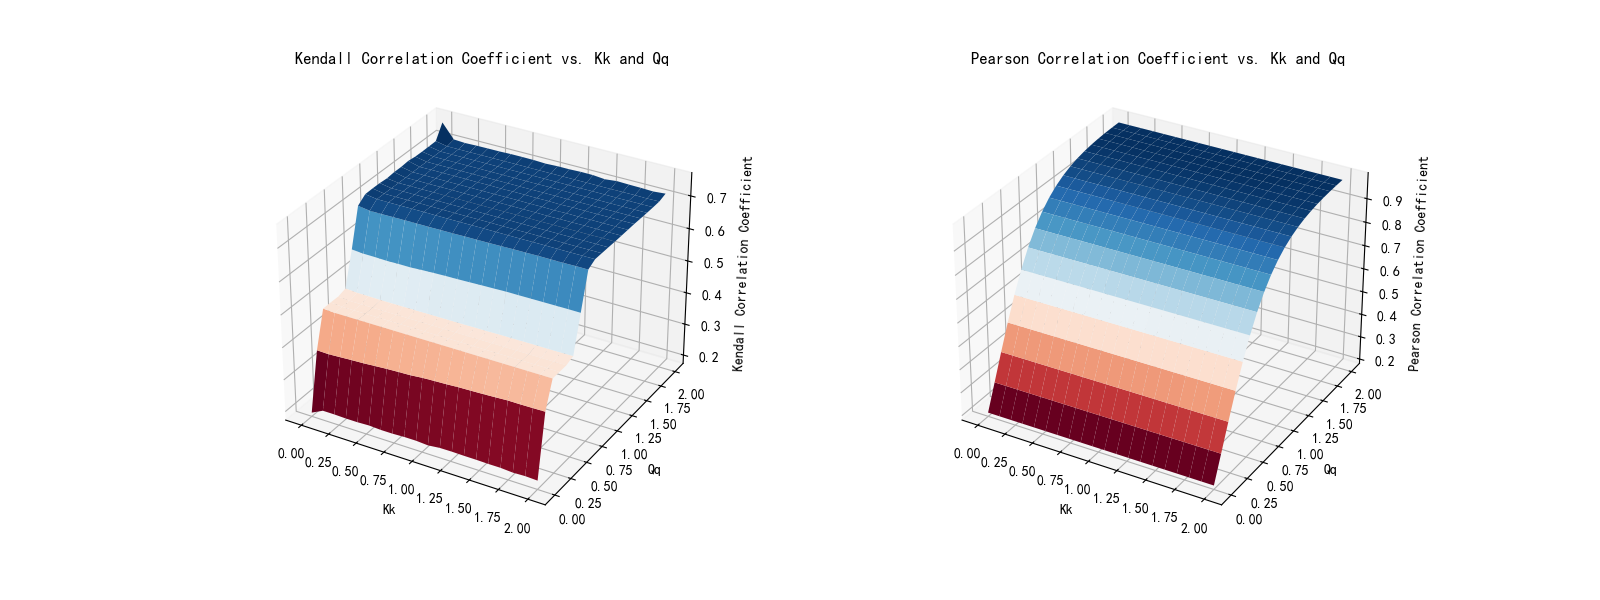
\includegraphics[width=.8\textwidth]{sensitive.png}
	\caption{Correlation Coefficient}\label{fig:sensitive}
\end{figure}

After k exceeds 0.9, similar effects are observed, and the coefficient does not consider the influence of dDELM on the correlation with winning or losing excessively. It can be considered that Kk has negligible impact on correlation after exceeding 0.9. Choosing 1 is more reasonable, and further adjustment is unnecessary. The chart shows that the influence of Qk is not significant, hence selecting a coefficient of 1 is more appropriate, and no further adjustment is required. This indicates that when k exceeds 0.9, the model is not sensitive to parameter changes and remains relatively stable.

\section{Model Evaluation}

\subsection{Advantage}
\begin{enumerate}[\bfseries 1.]
	\item Use the ARIMA time series model to forecast the trend of momentum (M). The differential analysis and shifting methods of the ARIMA time series model are particularly effective in short-term forecasting of trends related to time factors, especially for trends with significant fluctuations.
	\item Utilize a logistic regression model under Bayesian spatiotemporal theory to assess the factors influencing M. Compared to using simple classification algorithms that treat volatility as a binary distribution, transforming our model into conditional probability provides some continuity to the dependent variable. Additionally, the model's identified influencing factors generally align with the model's prior assumptions, indicating good predictive performance.
	\item Employ cross-validation to evaluate the first two models, thereby improving and optimizing our models for greater stability and generality. Post-validation, our model achieves a prediction accuracy of 93.17\% on other datasets. Sensitivity analysis indicates that our model exhibits good generalization capability.
	\item The momentum expression we propose encompasses the Score, Strength, and Server (3 S)—quantities with clear intuitive relevance to the outcome. We also creatively introduce a fatigue index based on running distance to better establish the momentum expression. The formulation is comprehensive and logically structured.
	\item Our preprocessing of raw data involves non-rigid quantization (normalization) and the substitution of dummy variables. The former ensures the generalization capability of the model under different scales (e.g., women's events), while the latter better captures the independent effects of different categories under a single variable.
\end{enumerate}

\subsection{Disavantage}
\begin{enumerate}[\bfseries 1.]
	\item The model's generalization can have a broader scope by refining the interaction between spatial factors (such as information about both teams and the venue) and temporal factors.
	\item The model exhibits a lag effect when predicting certain data and is less sensitive to data with low volatility.
\end{enumerate}


% 以下为信件/备忘录部分,不需要可自行去掉
% 如有需要可将整个 letter 环境移动到文章开头或中间
% 请在第二个花括号内填写标题,如「信件」(Letter)或「备忘录」(Memorandum)
\begin{letter}{Memorandum}
\begin{flushleft}  % 左对齐环境,无首行缩进
\textbf{To:} Coaches\\
\textbf{From:} Team 888888\\
\textbf{Date:} February 5th, 2024\\
\textbf{Subject:} Enhancing Athlete Performance in Matches through Momentum
\end{flushleft}

In modern professional tennis competitions, players have gained significant experience in their pre-match preparations and tactical planning. Through systematic physical training and cleverly designed game strategies, they ensure that they can perform at their best on the court. However, with the continuous improvement of athletic levels and increasingly fierce competition, relying solely on traditional preparation methods is no longer sufficient. Even the most outstanding professional players may experience fluctuations in their performance and could be overturned in seemingly advantageous situations. We introduce a new metric, momentum, which can comprehensively integrate various aspects of a player's performance, adapt effectively, and accurately predict the next game's fluctuations. This, in turn, allows for the analysis of an athlete's matches and the formulation of targeted recommendations to enhance their performance in games.

After establishing and improving our model and discussing the relationship between influencing factors and outcomes, we have determined that there is a strong correlation of up to 90\% between the first-order difference in momentum between two players and the outcome of the match, with a positive value indicating a higher likelihood for the player to score in the next point. Additionally, momentum can effectively consolidate various performance metrics used to evaluate a player's on-court performance and process them to determine the impact of different factors on a player's performance. This helps coaches provide tailored guidance to the athletes.

Based on the data from the 2023 Wimbledon Men's Tennis Tournament, we have found that momentum is primarily correlated with a player's confidence. When a player is on a winning streak or in an advantageous serving situation, their momentum tends to increase significantly. Conversely, when a player experiences consecutive losses or makes serving errors, their momentum tends to decrease significantly. In addition to this, objective factors such as the level of physical fatigue and the characteristics of the playing surface can also influence a player's condition and momentum.

\end{letter}


\newpage

% 参考文献
\begin{thebibliography}{99}
	
\bibitem{1} Trafimow, D. (2017) Why It Is Problematic to Calculate Probabilities of Findings Given Range Null Hypotheses. Open Journal of Statistics, 7, 483-499.\url{https://doi.org/10.4236/ojs.2017.73034}.	

\bibitem{2} Braidwood, J. (2023), Novak Djokovic has created a unique rival – is Wimbledon defeat the beginning of the end, The Independent.

\bibitem{3} Headrick, T. (2016) A Note on the Relationship between the Pearson Product-Moment and the Spearman Rank-Based Coefficients of Correlation.\url{http://dx.doi.org/10.4236/ojs.2016.66082}.

\bibitem{4}BOX G E P,JENKINS G M. Time series analysis forecasting and control(Rev ed) [ J] . Journal of Time,1976, 31( 4) :238-242

\bibitem{5} Ahn, H. (2014) Effect Modeling of Count Data Using Logistic Regression with Qualitative Predictors. Engineering, 6, 758-772. \url{http://dx.doi.org/10.4236/eng.2014.612074}.

\bibitem{6} Besag J, Mollié Y A. Bayesian image restoration, with two applications in spatial statistics[J]. Annals of the Institute of Statistical Mathematics, 1991, 43: 1-20. [48] Bernardinelli L 

\bibitem{7} Clayton D, Pascutto C, et al. Bayesian analysis of space-time variation in disease risk[J]. Statistics Medicine, 1995, 14(21-22): 2433-43

\bibitem{8} Heinz Kleinoder. The ITF coaching\&sport science review. The year issue 24.July2001

\bibitem{9} Nick Bollettieri. Keep score in mind-play your game accordingl y. Tennis magazin e,2007

\bibitem{10} Barnett, Tristan and Pollard, Graham (2007) How the tennis court surface affects player performance and injuries.* Medicine and Science in Tennis, 12 (1). pp. 34-37. ISSN 1567-2352 \url{https://www.independent.co.uk/sport/tennis/novak-djokovic-wimbledon-final-carlos-alcaraz-b2376600.html} 


















\end{thebibliography}

\end{document}  % 结束